\documentclass[12pt]{amsart}   % LaTeX with AMS style; 12 point for old eyes

\usepackage{paper}

\begin{document}

\graphicspath{ {figures/} }

\title[Shape of Stones]{Continuous and Discrete Models for Simulating Stone Erosion}
 
\author{Jonathan Allen, John Wang}
\date{\today}

\maketitle

\subsection*{Abstract}

In this paper we explore various techniques for modeling erosion processes on a stone. We develop and analyze an algorithm for modeling chipping by representing a stone as a polygon. We also develop a method for modeling gradual stone erosion through a Fast Fourier Transform (FFT) representation of a stone.

\section{Introduction}
Stones in riverbeds and on the ocean floor have very distinct shapes and contours. These stones tend to be smooth and flat, but the reason for this is not obvious. This paper examines how erosion affects the shape of stones. In particular, we examine two different mechanisms for stone erosion, a discrete one and a continuous one, and produce models for each one.

The first mechanism we study is the chipping of stones. One can imagine stones in a riverbed being tossed around and colliding with other stones. We create a discrete, polygonal model of a stone and a means of chipping the stone through a shear force. This model predicts that stones will tend to be flat and elongated.

The second mechanism we study is the wearing down of stones by gradual erosion. This mechanism appears when stones are gradually worn away by sand, water, or some other agent. We start of with a simple smooth model of the stone using spectral methods with the Fast Fourier Transform. This leads to problems, since the size of the stone decreases over time and changes shape, so we need to somehow resample. Most of our work involves designing a method for this resampling, which we are succesful at doing. We are then able to demonstrate our continuous model on a few simple problems, namely the processes of smoothing a stone and the process of erroding a stone from the bottom.


\section{Discrete Model}
In this section, we shall describe a model for simulating the chipping of a stone. In particular, we think of the erosion of a stone as coming from shear forces. This discrete model for eroding the stone allows us to simulate random processes and view the shape of a stone after some number of time steps. We provide computer simulations for the erosion process and analyze the model through these simulations.

\subsection{Shearing Stones}

The discrete model for stone erosion is based on the idea that stones are eroded via chipping. The process of chipping is analogous to dropping a stone from a specified height and applying a shear force to a particular point on the stone. Intuitively, one can think of a stone in a stream being eroded by being tossed and turned by the force of the river. This tossing and turning causes the stone to collide with other stones on the bottom of the riverbed, causing chipping to occur.

We model the interaction between two stones as a shear force, a force that causes two parts of a stone to move in opposite directions. The point where a stone collides with another stone is the point where the shear force is concentrated. This causes the stone to break into two pieces. The processes by which shear forces cause breakages in materials are extremely complicated, so we will use the following simple assumption: we shall assume that the amount of volume that is sheared off of a stone is proportional to the amount of force incident on the stone.

\subsection{Definitions}

This section will define how we represent a stone in the discrete model. We will represent a stone as a polygon in $k$-dimensional space with $n$ vertices.

\begin{definition}
  A polygon $s$ consisting of $n$ vertices is defined by the set of vertices $s = \{ \bvec{v}_0, \ldots, \bvec{v}_{n-1} \}$ where each vertex $\bvec{v}_i \in \mathrm{R}^k$ is a tuple. Vertices $\bvec{v}_i$ and $\bvec{v}_{i+1}$ are connected by a line segment for all $i \in \{0, 1, \ldots, n \}$ and the line segments do not intersect each other, except at the vertices.
\end{definition}

When referring to vertices, we will use the convention of taking vertex indices modulo $n$ for convenience. Hence $v_{i \mod{n}} \equiv v_i$. Note that this means that $v_{n} = v_{0}$ so that vertex $v_{n-1}$ has a line segment connecting it to $v_{0}$.

The centroid $\bvec{c}_s$ of a stone $s$ is the center of mass of the stone when the stone has uniform density. In other words, the centroid is the point $\bvec{c}_s \in \mathrm{R}^k$ where the following holds:

\begin{eqnarray}
 \int_V (\bvec{r} - \bvec{c}_s) dV = 0
\end{eqnarray}

Where $V$ is the area of the stone, using all values $\bvec{r} \in V$. 

In addition, we will define a pseudo-probability distribution, which we will use to generate random points on a line.

\begin{definition}
  A pseudo-probability distribution $\mathrm{P}(x, y)$ defines $Pr[i | \mathrm{P}]$, the probability of selecting some $i \in \mathrm{R}$, such that $Pr[i | \mathrm{P}] = 0$ for $i \notin [x,y]$ and $\int_{x}^y Pr[i | \mathrm{P}] di = 1$. We use the notation $j \sim \mathrm{P}(x,y)$ to denote that $j \in [x,y]$ is a realization of a draw from the pseudo-probability distribution $\mathrm{P}(x,y)$. In other words, we select $j$ with probability $Pr[j | \mathrm{P}]$.
\end{definition}

For example, one possible pseudo-probability distribution $\mathrm{P}(x,y)$ would have $Pr[i | \mathrm{P}] = \frac{1}{y-x}$ for all $i \in [x,y]$. This would be the uniform pseudo-probability distribution on a range $[x,y]$.

We will also introduce the notion of a convex vertex, which will be useful when defining our chipping process.

\begin{definition}
  A convex vertex $\bvec{v}_c$ on a polygon $s$ consisting of $n$ vertices is a vertex $\bvec{v}_i$ which, when removed from the polygon $s$ to create a new polygon $s' = \{ \bvec{v}_0, \ldots, bvec{v}_{i-1}, \bvec{v}_{i+1}, \ldots, \bvec{v}_{n-1} \}$ has the property $V(s) \geq V(s')$ (where $V(\cdot)$ denotes the volume of a stone).
\end{definition}

In the following sections, we will assume that one cannot chip a vertex which is not convex. The reasoning relies on our intuition for how a stone chips. Non-convex vertices can be thought of as moving in towards the center of a stone, and chipping a stone can be thought of being caused by the stone crashing into the ground. It is impossible for a stone to be chipped on a vertex which is not convex if the stone is falling onto a flat surface (the protruding vertices surrounding the convex vertex will be chipped first). Therefore, we make the assumption that convex vertices are the only ones which can be chipped through our mechanism.

\subsection{The Chipping Process Model}

With this in mind, we shall now develop a model for the chipping of a stone based on shearing. We will confine our work to $\mathrm{R}^2$. The main idea of the model is that we will represent a stone as a two-dimensional polygon, and chip off a constant amount of area of the stone at every time step. In this way, we will attempt to capture the process of a stone colliding with another stone on a riverbed. Randomness will be introduced into the model by randomly selecting somewhere on the stone to start the shearing.

We shall now give a formal definition of the chipping process. A chip for a pseudo-probability distribution $\mathrm{P}(0,1)$, stone $s$, and area $A$ is denoted $Chip(\mathrm{P}, A, s)$ and is represented as follows:

\begin{enumerate}
  \item Select a vertex $\bvec{v}_j$ from $s$. To select this vertex, we find the centroid $\bvec{c}_s$ of stone $s$ and choose an angle $\gamma \in [0, 2\pi)$ uniformly at random. Now, define the ray $\bvec{l}$ as the ray with an initial point of $\bvec{c}_s$ which extends outwards infinitely at an angle of $\gamma$ from the horizontal. The vertex with the minimum perpendicular distance to $\bvec{l}$ will be $\bvec{v}_j$. Repeat this process as many times as necessary until we have selected a convex vertex.
  \item Given vertex $\bvec{v}_j$, define $\bvec{l}_l$ as the line segment which connects $\bvec{v}_j$ and $\bvec{v}_{{j-1}}$. Similarly, define $\bvec{l}_r$ as the line segment connecting $\bvec{v}_j$ and $\bvec{v}_{{j+1}}$ (recall that our convention is to take the vertex indices modulo $n$).
  \item Select $\bvec{l}_1$ from the set $\{ \bvec{l}_l, \bvec{l}_r \}$ uniformly at random (i.e. $Pr[\bvec{l}_1 = \bvec{l}_l] = Pr[\bvec{l}_1 = \bvec{l}_r]$). Call the line segment which was not selected $\bvec{l}_2$.
  \item Select a point $\bvec{p}_1$ at random from $\bvec{l}_1$. To do this, we select a random $t \sim \mathrm{P}(0,1)$ and let $\bvec{p}_1 = \bvec{v}_j t + (1-t) \bvec{v}_{{j-1}}$. Recall that $t \sim \mathrm{P}(0,1)$ denotes that $t$ is drawn from the pseduo-probability distribution $\mathrm{P}(0,1)$.
  \item Select the point $\bvec{p}_2$ which lies on $\bvec{l}_2$ for which the polygon defined by $\{\bvec{p}_1, \bvec{v}_j, \bvec{p}_2\}$ has an area of $A$. If no such polygon exists, then choose $\bvec{p}_2 = \bvec{v}_{{j+1}}$.
  \item Create a new stone $s'$ whose vertices are given by
    \begin{eqnarray*}
      s' = \{ \bvec{v}_1, \ldots, \bvec{v}_{j-1}, \bvec{p}_1, \bvec{p}_2, \bvec{v}_{j+1}, \ldots, \bvec{v}_n \}
    \end{eqnarray*}
    Here, the vertex $\bvec{v}_j$ has been replaced by $\bvec{p}_1$ and $\bvec{p}_2$ in the list of vertices for $s$. The new stone $s'$ now has one more line segment and vertex than the old stone $s$.
\end{enumerate}

Now that we have defined a chip $Chip(\mathrm{P}, A, s)$, we can define our entire model as a chipping process.

\begin{definition}
A chipping process for a probability distribution $\mathrm{P}$, stone $s$, area $A$, and iterations $k$ is denoted $ChipProcess(\mathrm{P}, A, s, k)$. A chipping process returns a stone $s'$ which has iteratively conducted $k$ chips. Thus, a chipping process takes a stone $s$ and creates $s_1 = Chip(\mathrm{P}, A, s)$, $s_2 = Chip(\mathrm{P}, A, s_1)$, \ldots, $s_k = Chip(\mathrm{P}, A, s_{k-1})$, and returns $s' = s_k$.
\end{definition}

\subsection{Simulations}

The chipping process model allows us to simulate changes to a stone. A stone which undergoes a chipping process should have a shape which is close to the stones which undergo erosion and chipping in the real world (if our chipping process model is an accurate description of erosion).

To examine the accuracy of our model, we performed computer simulations using the Python programming language and the Shapely library. With computer simulations, we were able to create multiple instances of a chipping process and analyze the shapes of the resulting stones. We were also able to use multiple probability distributions $\mathrm{P}$ and areas $A$ to generate different chipping processes.

\begin{figure}
  \begin{center}
    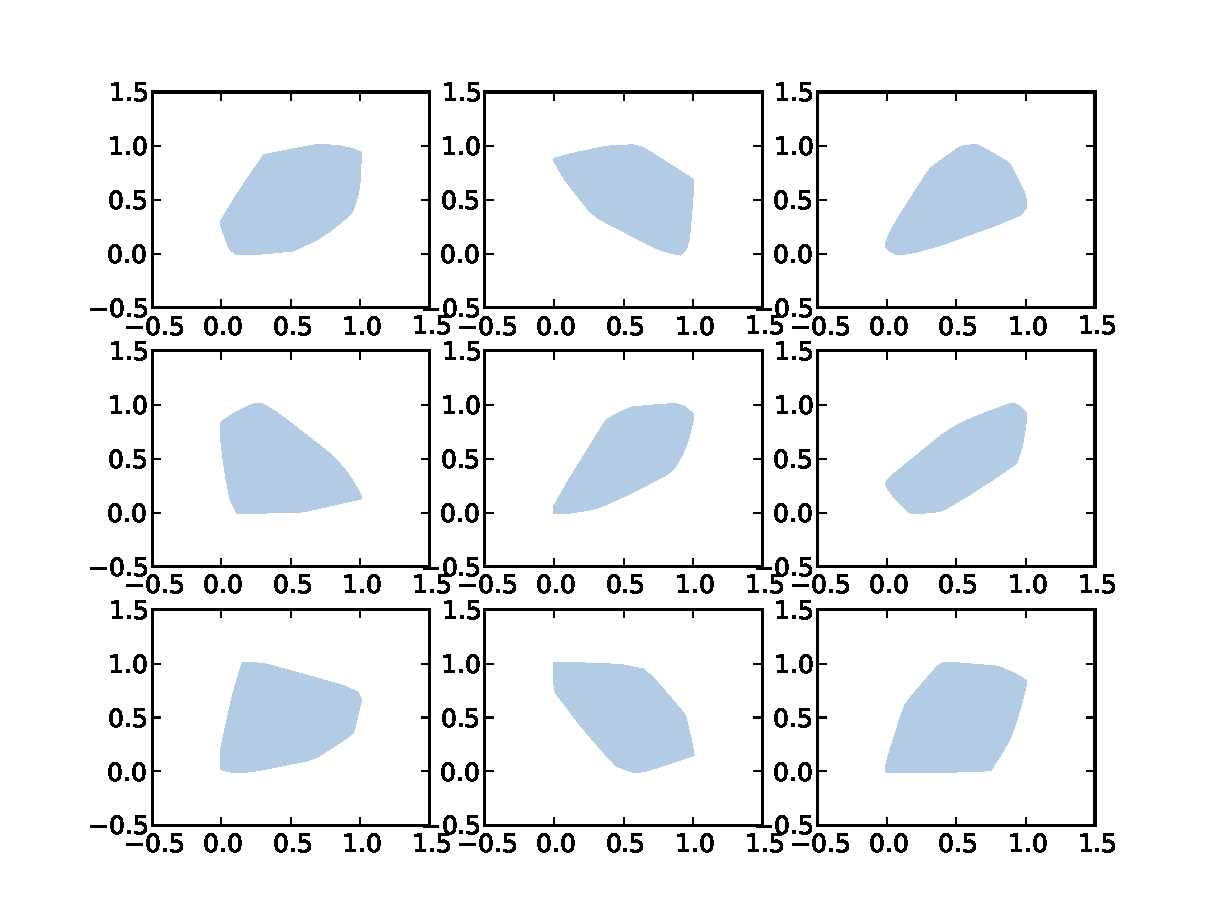
\includegraphics[width=4in]{area_chipper_sample.pdf}
  \end{center}
  \caption{Chipping Process for a Unit Square \label{fig:area_chipper_sample}}
\end{figure}


For our simulations, we use a pseudo-probability distribution $\mathrm{P}(0,1)$ which is a normal distribution with mean $\mu$ and standard deviation $\sigma$. We select $\mu \in [0,1]$ and all realizations of the normal distribution which fall outside of $[0,1]$ are discarded and we select a new element from the normal distribution. We will denote a pseudo-probability distribution which is using a normal distribution with $\mathrm{P}(0,1) = \mathrm{N}(\mu, \sigma)$.

Figure \ref{fig:area_chipper_sample} shows the results for nine chipping process runs. The parameters used in these runs were $\mathrm{P} = \mathrm{N}(0.5, 0.15)$, $A = 0.05$, $k = 50$, and $s = \{(0,0), (1,0), (1,1), (0,1)\}$. The chipping processes each started out with a stone which was a unit square. The stones were chipped 50 times by the method described by the model. The probability distribution $\mathrm{P}$ is a normal distribution so that $t = 0.5$ is the most likely $t$ to choose. In other words, it is most likely that $\bvec{p}_1$ will be chosen as the midpoint of the line segment $\bvec{l}_1$.

This distribution was chosen because it is more likely that shear forces will cause a symmetric split about the vertex $\bvec{v}_j$. However, it is still possible for non-symmetric splits to occur, i.e. when $t \neq 0.5$. The normal distribution captures this nicely (all realizations of $t$ which are not in the interval $[0,1]$ were discarded).

Figure \ref{fig:area_chipper_sample} displays the typical results of the chipping process model. None of the stones resemble a square and it would be hard for anyone to have guessed that these shapes came from a common origin. In fact, the randomization from the distribution $\mathrm{P}$ makes all of the shapes slightly different.

To examine the chipping process more closely, we can look at how circular or elliptical the resulting shapes are. One would expect rocks in a stream or riverbed to be elliptical in shape. We can therefore examine the distance of random points on a stone from the centroid. We will generate a large number of random points, and plot their distances from the centroid.

More precisely, a random point $\bvec{p}_s$ on the stone $s$ will be selected by the following process:
\begin{enumerate}
  \item Produce a random angle $\theta \in [0, 2\pi)$, drawn uniformly from the range $[0, 2\pi)$.
  \item Draw a ray from the centroid of the stone with an angle $\theta$ from the horizontal (x-axis).
  \item The ray will intersect with the stone in exactly one location (since the stone is closed). Set the random point $\bvec{p}_s$ as the point where the ray intersects an edge on the stone.
\end{enumerate}

When we plot the distances, we will scale the distances to the centroid of a point $\bvec{p}_s$, denoted by $d(\bvec{p}_s, \bvec{c}_s)$. We will sample $q$ random points from the stone, and plot the scaled distances. Let $\min_d = \min d(\bvec{p}_s, \bvec{c}_s)$ be the minimum observed distance and $\max_d = \max d(\bvec{p}_s, \bvec{c}_s)$ be the maximum observed centroid distances for the $q$ samples on a stone $s$. We will define the scaled distance to the centroid of a stone $s$ as $d'_s(\bvec{p}_s, \bvec{c}_s)$ with the following formula:

\begin{eqnarray}
  d'_s(\bvec{p}_s, \bvec{c}_s) = \frac{d(\bvec{p}_s, \bvec{c}_s) - \min_d}{ \max_d - \min_d }
\end{eqnarray}

We can get intuition for this metric by examining common shapes. In a circle, all of the distances to the centroid would be the same. In an elipse, one would expect a skewed curve, with more points lying closer to the centroid. One can see this by examining all points on an ellipse which have distances from the centroid lying in $[d, d + \epsilon]$. The slices of the ellipse which are carved out will have strictly greater total angle than the angles carved from using distances in $[d + \epsilon, d + 2 \epsilon]$.

\begin{figure}
  \begin{center}
    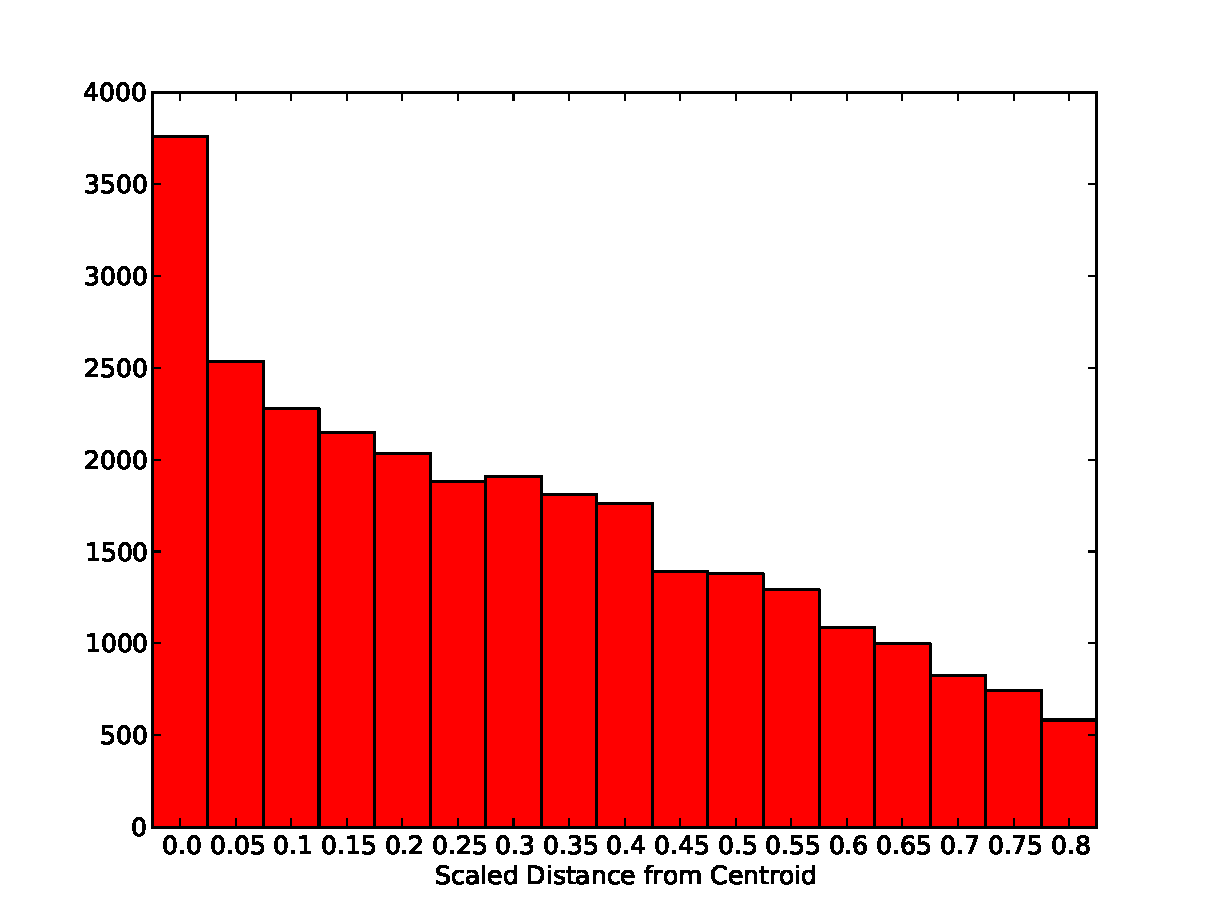
\includegraphics[width=4in]{distance_from_centroid.pdf}
  \end{center}
  \caption{Histogram of Vertex Distance From Centroid \label{fig:distance_from_centroid}}
\end{figure}

Figure \ref{fig:distance_from_centroid} shows the distribution of vertex distances which were simulated with the same parameters as used for figure \ref{fig:area_chipper_sample}. One can see that the distribution is skewed, with most points being closer to the centroid. The distribution of vertex distances from the centroid show that the shapes that result from this set of chipping process conditions have a similar distribution as an ellipse would.


\section{Continuous Model}
\subsection*{Method}

We next moved on to develop a continuous surface erosion model. Physically this model represents a surface being worn down, such as a bar of soap in water or ice melting. 

There are a wide range of different erosion processes, and most of them are very complex. To simplify our models, all of our processes erode (move) each point along the surface in a direction normal to the surface at the point. This rarely happens in real life, because of non-homogeneous materials, nonlinear behavior, etc., but it is a reasonable assumption to make for a simplified model.

Rather than modeling erosion as a discrete process, as was done in the previous section, we can model it with the following differential equation

\begin{equation}
\label{eq:erosion-diff-eq}
\frac{d\bvec{x}}{dt} = g(\bvec{x}) \; \bhat{n}(\bvec{x})
\end{equation}

for some function $g(\bhat{x})$ to be defined shortly. $\bhat{n}(\bvec{x})$ is the unit vector normal to the surface at $\bvec{x}$.

The method used to represent the continuous surface will be explained momentarily, but first we will take a moment to explain the various erosion processes that we modeled.

The first process is a soap bar being worn down by a person holding it in their hand, which we will call our \textit{smoothing model}. In this process, the corners of the soap bar will get worn down quickest, because they are the first parts of the surface to come into contact with the person's hand. Technically the furthest protruding bumps will be worn down quickest, but to simplify the problem, we consider every point of the surface to wear down at a rate proportional to the curvature at the point. We will use a signed curvature, so that positive curvature represents an outward facing bump, and negative curvature represents an indentation in the surface. $g(\bvec{x})$ for this model is the following ($\kappa$ is the curvature)

\begin{equation}
g(\kappa(\bvec{x})) = \tan^{-1}(\beta \, (\kappa(\bvec{x}) - \alpha)) + \frac{\pi}{2}
\end{equation}

For our model we chose parameters, $\alpha = 1, \; \beta = 5$.

Our second process is an object sitting in a bath of acid, which we will call our \textit{bottom recession model}. In this process, the bottom of the object will recede quickest. $g(\bvec{x})$ for this model is the following ($x_{2, min}$ is the lowest point on the object)

\begin{align}
  f(\bvec{x})& = \frac{1}{\alpha \, (x_2 - x_{2, min}) + \beta} - \gamma\\
  g(\bvec{x})& = \begin{cases}
    f(\bvec{x}) \qquad &\text{for} \quad f(\bvec{x}) > 0\\
    0 \qquad &\text{otherwise}
  \end{cases}
\end{align}

For our model we chose parameters, $\alpha = 10, \; \beta = \gamma = 0.1$.

\subsection*{Example Surface}

The example shape that we will use is shown in Figure \ref{fig:blob-shape}.

\begin{figure}[H]
    \begin{center}
      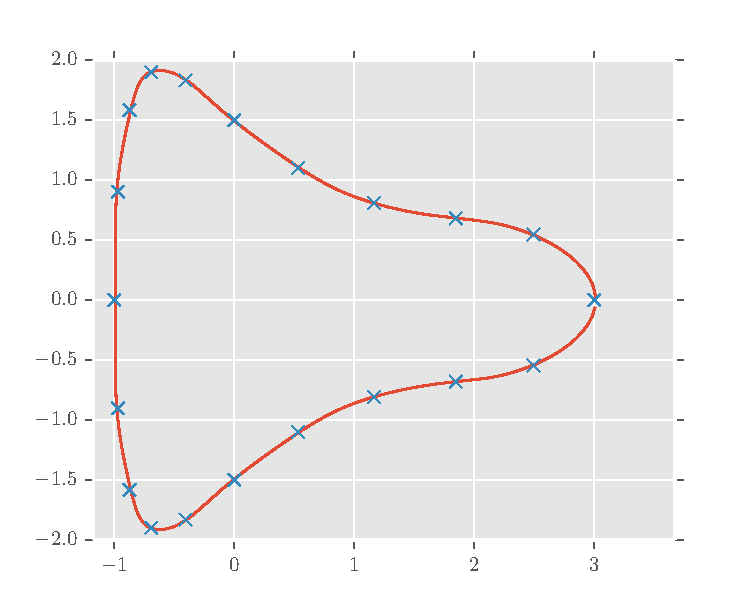
\includegraphics[keepaspectratio]{blob_shape.pdf}
    \end{center}
  \vspace{-.2in} % corrects bad spacing
  \caption{\label{fig:blob-shape} Example shape.}
\end{figure}

The equations for the shape are the following ($T_i$ is the i\textsuperscript{th} Chebyshev polynomial)

\begin{align*}
  x_1(s) = \cos(s) \paren{2 T_0(\paren{\frac{s-\pi}{\pi}}) + T_2\paren{\frac{s-\pi}{\pi}}}\\
  x_2(s) = \sin(s) \paren{2 T_0(\paren{\frac{s-\pi}{\pi}}) + T_4(\paren{\frac{s-\pi}{\pi}})}
\end{align*}

\subsection*{Surface Equations}

Our surface is modeled with two vectors, $x_1, x_2 \in \R^N$ for some resolution $N$. Then $\bvec{x} \coloneqq \bracket{x_1^T, x_2^T}$, with $x_1$ and $x_2$ being the two coordinates of points sampled counterclockwise along the surface.

\begin{align}
  \dot{\bvec{x}}& \coloneqq \frac{d\bvec{x}}{dt} \tag{Velocity}\\
  \ddot{\bvec{x}}& \coloneqq \frac{d^2\bvec{x}}{dt^2} \tag{Acceleration}\\
  \kappa& = \frac{\dot{\bvec{x}} \times \ddot{\bvec{x}}}{\dot{x}^3} \tag{Curvature}
\end{align}

\subsection*{Numerical Modeling}

We chose to model the surface parametrically with a Discrete Fourier series using spectral methods. Our processes tend to smooth the surfaces out over time, so spectral methods would capture this much better than a local approximation of the surface using finite differences which only act locally at points. All of our surface are in $\R^2$, so we will use the Real Fast Fourier Transform (equations in the appendix). The following equations are derived in most introductory spectral method texts, so they will be stated without proof here

\begin{align}
  \dot{\bvec{x}}& = RFFT^{-1}\paren{diag(i \, [0:N/2, 0]) \; RFFT(\bvec{x})}\\
  \ddot{\bvec{x}}& = RFFT^{-1}\paren{diag(i^2 [0:N/2, 0]^2) \; RFFT(\bvec{x})}
\end{align}

Note: $diag(\bvec{a})$ is the diagonal matrix with the elements of $\bvec{a}$ along the diagonal.

Using the FFT, the surface normal and curvature can now be easily found

\begin{align}
  \bhat{n}& = [-\dot{x}_2, \dot{x}_1]\\
  k& = \frac{\dot{x}_1 \ddot{x}_2 - \dot{x}_2 \ddot{x}_1}{\paren{x_1^2 + x_2^2}^{3/2}}
\end{align}

\subsection*{Point Collision Problems}

Unfortunately, the simplicity gained from modeling the surface with Fourier series is lost when the surface starts to shrink. As can be seen in Figure \ref{fig:remove-lowest-blob-bad}, the process works well for a short time period, but over time a sharp point, and the surface actually folds over itself (a physical impossibility).


\begin{figure}[H]
    \begin{center}
      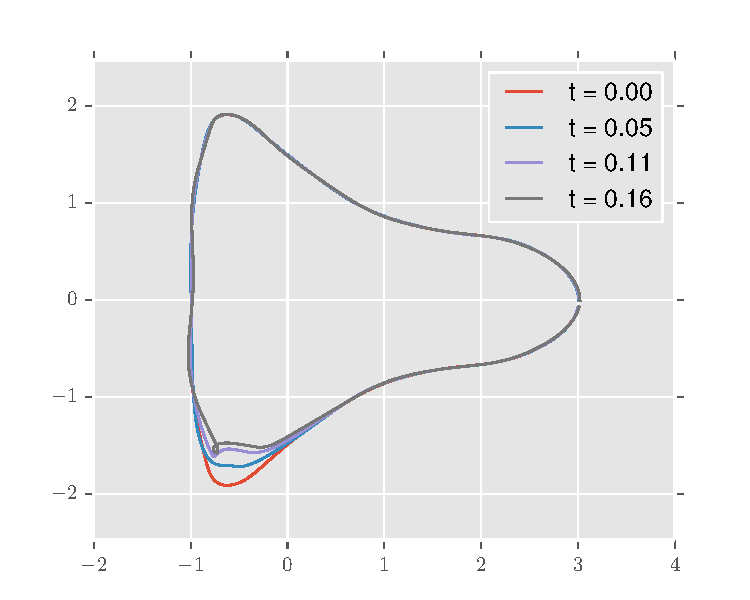
\includegraphics[keepaspectratio]{remove_lowest_blob_bad.pdf}
    \end{center}
  \vspace{-.2in} % corrects bad spacing
  \caption{\label{fig:remove-lowest-blob-bad}}
\end{figure}

To see why this occurs, we will show a zoomed in portion of the same figure, but with the evaluation points shown. 

\begin{figure}[H]
    \begin{center}
      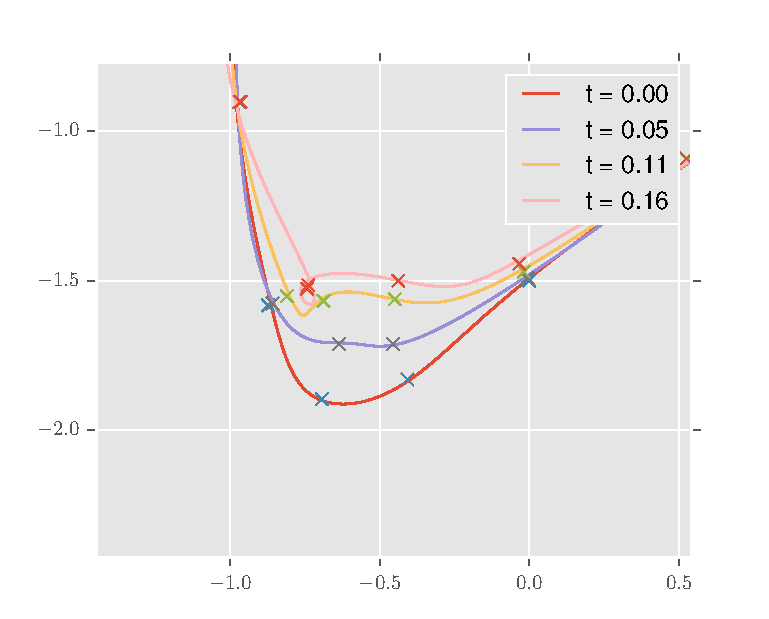
\includegraphics[keepaspectratio]{remove_lowest_blob_bad_zoom.pdf}
    \end{center}
  \vspace{-.2in} % corrects bad spacing
  \caption{\label{fig:remove-lowest-blog-bad-zoom}}
\end{figure}

Looking closely, it can be seen that the sharp corner forms when evaluation points get too close to each other. Our guess is that this occurs because we are using discrete time stepping, so there are errors in the approximation of the shape's change with time. This is fine when the evaluation points are far from each other, but when they get close to each other, the errors become significant and affect the direction of the surface unit normal vectors. 

\subsection*{Redistributing Points}

The most obvious way to fix this problem would be to redistribute the points evenly on the surface at every step. This wouldn't be too difficult of a task, since we can easily integrate with the FFT. 

Unfortunately, if we arbitrarily move points around, we lose spectral accuracy. Spectral methods . This method turns out to work, but I will hold off explaining it 

\subsection*{High Frequency Damping}

Our first approach to improve the algorithm was to use fewer Fourier terms than evaluation points, in an attempt to better approximate the shape while ignoring the higher frequencies. This unfortunately performed even worse than our original algorithm.

\subsection*{Partial High Frequency Damping}

In the \textit{bottom recession model}, $x_1$ should be changing slowly and smoothly with time, since the recession model primarily moves points upwards. In Figure \ref{fig:remove-lowest-blob-bad-x}, $x_1$ is plotted, and we can see that this is not the case in our simple algorithm and large high frequency oscillations appear as time increases. 

\begin{figure}[H]
    \begin{center}
      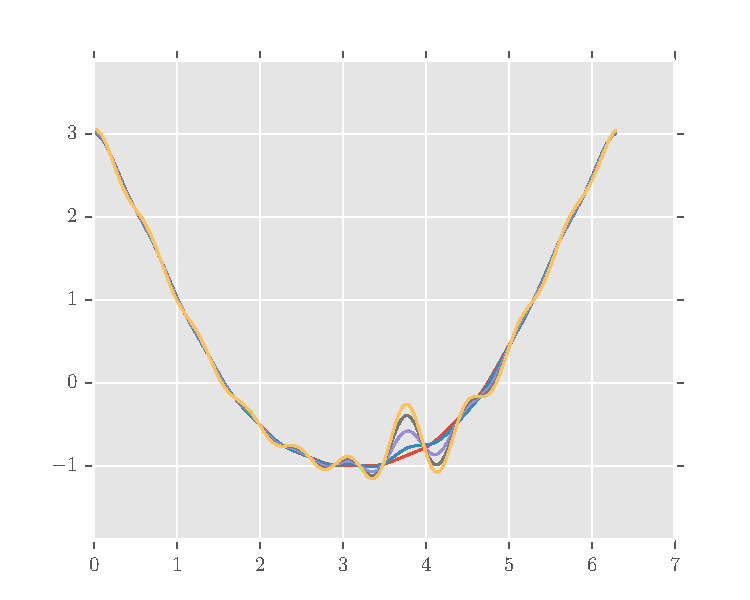
\includegraphics[keepaspectratio]{remove_lowest_blob_bad_x.pdf}
    \end{center}
  \vspace{-.2in} % corrects bad spacing
  \caption{\label{fig:remove-lowest-blob-bad-x}}
\end{figure}

This led us to try to artificially dampen the high frequencies in $x_1$, by manually zeroing out the high frequency Fourier coefficients. This worked reasonably well, but was not a very robust method. Our shape is nice, because $x_1$ can be represented accurately with very few Fourier terms, but this would not be the case for more complicated shapes and other models, such as the \textit{smoothing model} that affects $x_1$ and $x_2$ equally. 

\subsection*{Continuous Redistribution}

To redistribute points, we need to find some smooth function that will map points spaced evenly on the surface to evenly distributed $theta$. This can be achieved by 

\begin{align}
  \frac{d\bvec{x}}{dt}& = g(x) \; \bhat{n} + f(\bvec{a}_t)\\
  \bvec{a}_t& = \frac{\ddot{\bvec{x}} \cdot \dot{\bvec{x}}}{\norm{\dot{\bvec{x}}}} \; \frac{\dot{\bvec{x}}}{\norm{\dot{\bvec{x}}}}
\end{align}

$\bvec{a}_t$ is the component of $\ddot{\bvec{x}}$ tangent to the surface. $\dot{\bvec{x}}$ is inversely proportional to the density of points on the surface. We want to shift points away from denser areas, which means moving in the direction of larger $\dot{\bvec{x}}$.

As can be seen in Figure \ref{fig:remove-points-blob-good}, this dramatically improves our algorithm.

\begin{figure}[H]
    \begin{center}
      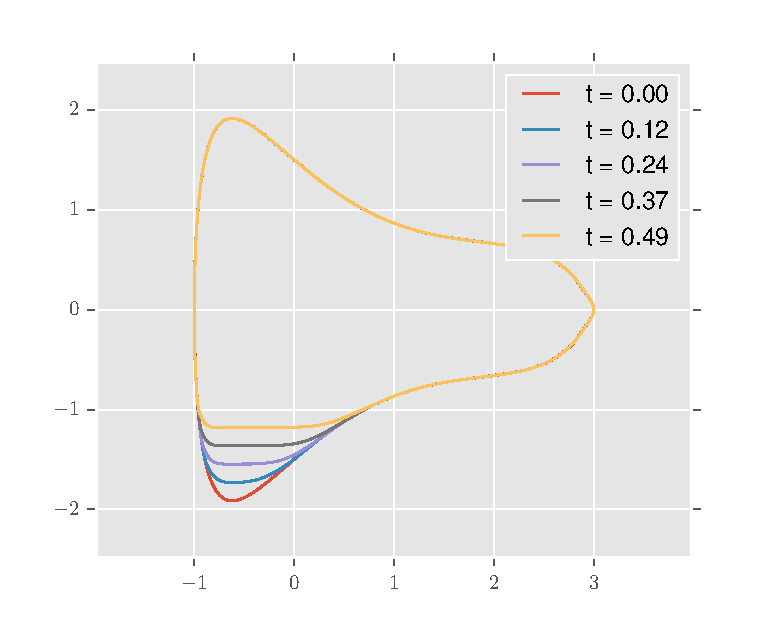
\includegraphics[keepaspectratio]{remove_points_blob_good.pdf}
    \end{center}
  \vspace{-.2in} % corrects bad spacing
  \caption{\label{fig:remove-points-blob-good}}
\end{figure}

If we plot the evaluation points (Figure \ref{fig:remove-points-blob-good-points}, it can be seen that the points redistribute themselves over time to stay evenly spaced on the surface.

\begin{figure}[H]
    \begin{center}
      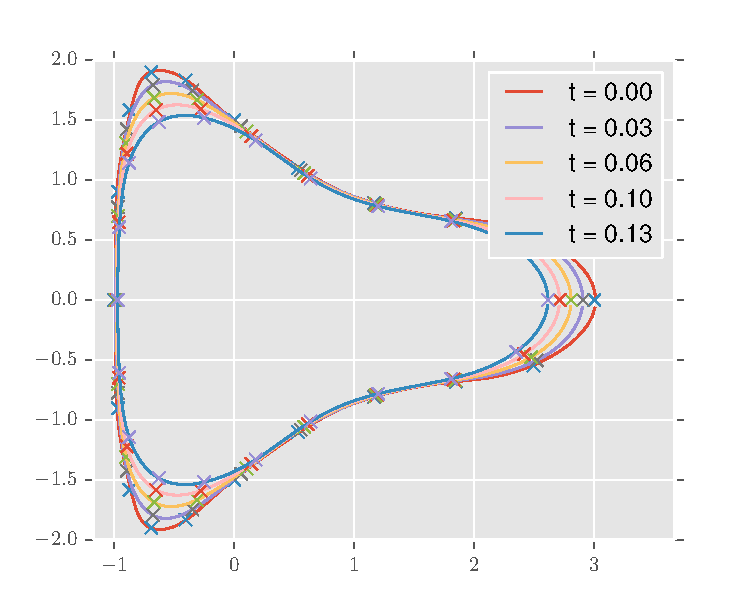
\includegraphics[keepaspectratio]{remove_points_blob_good_points.pdf}
    \end{center}
  \vspace{-.2in} % corrects bad spacing
  \caption{\label{fig:remove-points-blob-good-points}}
\end{figure}


\section*{Appendix}

\subsection*{Real Fourier Transform}

The Real Fourier transform is defined as

\begin{align*}
  \bhat{x} \coloneqq RFFT(x)_k\\
  & \coloneqq \sum_{n=0}^{N-1} e^{-2\pi i k (n/N)} x_n \qquad \text{for} \quad k = 0, \dotsc, N/2+1
\end{align*}

Note: the terms $FFT$ and Fourier transform are used interchangeably in the paper. Technically they are not synonyms, but it is common practice to use the terms interchangeably.

And the inverse transform is defined as

\begin{align*}
  x& \coloneqq RFFT^{-1}(\bhat{x})\\
  & \coloneqq \frac{1}{N} \paren{\sum_{k=0}^{N/2+1} e^{2\pi i k (n/N)} X_k + \sum_{k=N/2+2}^{N-1} e^{2\pi i k (n/N)} \bar{X}_k} \qquad \text{for} \quad n = 0, \dotsc, N-1
\end{align*}

\section{Conclusion}
In this paper, we presented two models which could determine how stones are shaped by erosion. The first model was a discrete model based off of a mechanism for chipping a stone via shear forces. The second model was a continuous model that used Fourier transforms to model a stone being worn down. Each model targets a different aspect of erosion, and taken together, one can better understand the actual mechanism for the erosion of stones.


\section*{Appendix}
\subsection*{Real Fourier Transform}

The Real Fourier transform is defined as

\begin{align*}
  \bhat{x} \coloneqq \mathcal{RFFT}(x)_k\\
  & \coloneqq \sum_{n=0}^{N-1} e^{-2\pi i k (n/N)} x_n \qquad \text{for} \quad k = 0, \dotsc, N/2+1
\end{align*}

Note: the terms $FFT$ and Fourier transform are used interchangeably in the paper. Technically they are not synonyms, but it is common practice to use the terms interchangeably.

And the inverse transform is defined as

\begin{align*}
  x& \coloneqq \mathcal{RFFT}^{-1}(\bhat{x})\\
  & \coloneqq \frac{1}{N} \paren{\sum_{k=0}^{N/2+1} e^{2\pi i k (n/N)} X_k + \sum_{k=N/2+2}^{N-1} e^{2\pi i k (n/N)} \bar{X}_k} \qquad \text{for} \quad n = 0, \dotsc, N-1
\end{align*}

\bibliographystyle{plain}
\begin{thebibliography}{9}
\bibitem{wikipedia_fft}
	Fast Fourier Transform. (2013, 10 8). Retrieved from Wikipedia: \url{http://en.wikipedia.org/wiki/Fft}
\bibitem{trefethen_2000}
	Trefethen, L. N. (2000). Spectral Methods in MATLAB. Philadelphia: SIAM.
\end{thebibliography}

\end{document}
